\subsection{Parser sensitivity and failure rates}
\label{sec:parser-results}

The parser affects the measured scores differently across benchmarks. GSM8K and Countdown rarely fail at the parser-entry stage, so their main errors are wrong answers, invalid equation chains, or missing required answer formatting. Trip Planning is different: many outputs are rejected before semantic scoring because the itinerary structure is malformed. For that benchmark, accuracy reflects both planning quality and compliance with the parser's expected format.

\begin{figure}[!htbp]
\centering
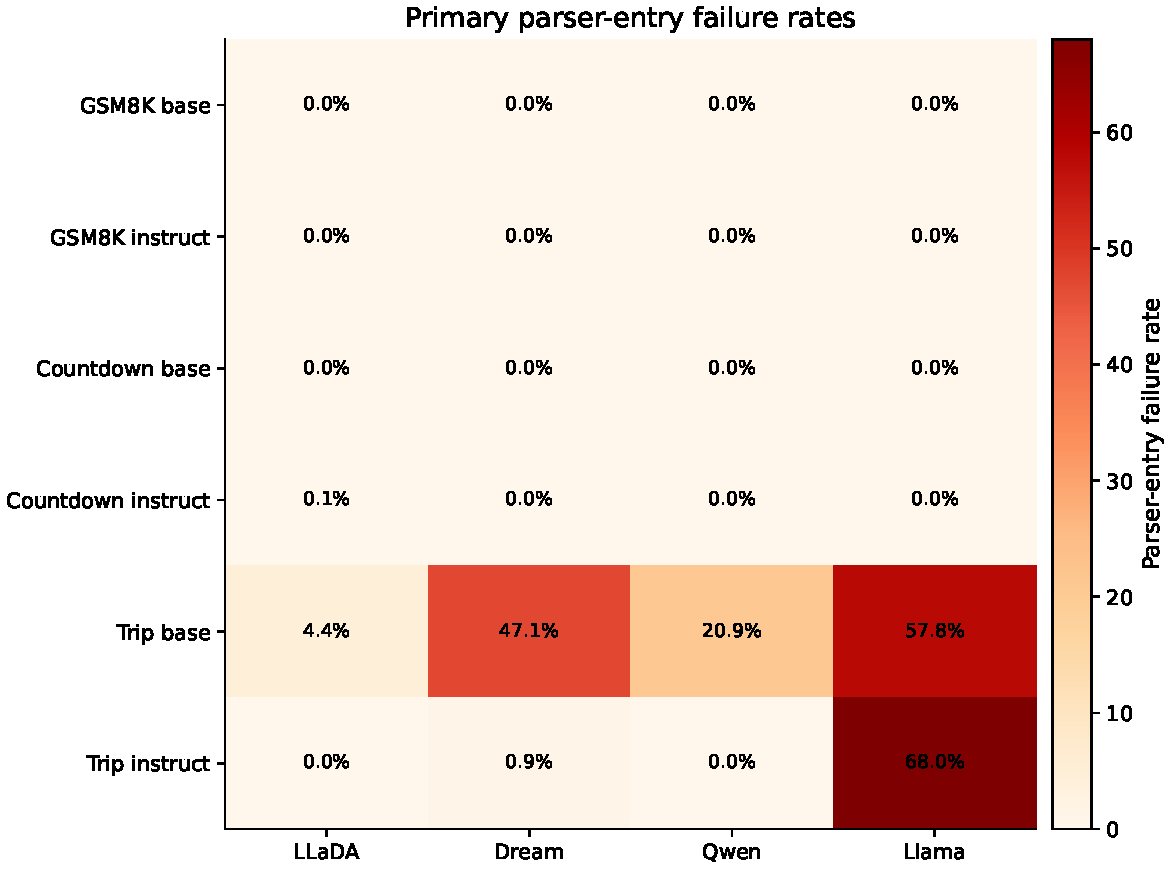
\includegraphics[width=0.9\textwidth]{images/parser_failure_rates.pdf}
\caption{Primary parser-entry failure rates for the six main comparison conditions. GSM8K and Countdown almost never fail at parser entry, while Trip Planning can be dominated by outputs that do not pass the itinerary parser's structural checks. For Trip Planning, these rates are the complement of the parseability column in Table~\ref{tab:trip-parseability-semantic}.}
\label{fig:parser-failure-rates}
\end{figure}

The sensitivity analysis is deliberately kept separate from the primary strict results. GSM8K parser crashes are rare in the main runs, but the permissive final-number scorer changes some measured scores, as shown in Table~\ref{tab:gsm8k-strict-vs-permissive}. Countdown behaves differently: parser-entry failures are effectively absent, and an alternate single-expression parser does not rescue additional correct samples because the main failure is semantic invalidity, especially wrong number use. Trip Planning is the parser-heavy task. In the main stochastic rows, Dream-Base has a $47.1\%$ primary-parser-entry failure rate and Llama-Base has $57.8\%$; Llama-Instruct under the templated prompt fails parser entry on $68.0\%$ of samples, while the flat Llama-Instruct run is much more parseable. Table~\ref{tab:trip-parseability-semantic} reports the same effect from the other direction: Trip parseability is $100\%$ minus the parser-entry failure rate, and semantic correctness is reported separately.
